%!TEX TS-program = xelatex
%!TEX root = ../../maxwell2018thesis.tex

\chapter[The Complex Searcher Model and Stopping Strategies]{The Complex Searcher Model\\and Stopping Strategies}\label{chap:csm}
In Part~\ref{part:intro}, we provided a comprehensive overview of the current state-of-the-art of user modelling within the field of~\gls{acr:iir} -- and stopping within search. In this chapter, we present an improvement on the current state-of-the-art, providing an outline of the main conceptual and theoretical contributions of this thesis, which include proposals of:

\vspace*{-2mm}
\begin{itemize}
    \item[\blueboxbold{(i)}]{a more complex and realistic user model -- the~\glsfirst{acr:csm} -- that captures the key interactions that take place during an~\gls{acr:iir} session (Section~\ref{sec:csm:csm}); and}
    \item[\blueboxbold{(ii)}]{an enumeration of a number of \emph{stopping strategies} that we will be evaluating (Section~\ref{sec:csm:stopping}).}
\end{itemize}
\vspace*{-2mm}

These outlines provide the foundations for the subsequent contributory chapters of this thesis that aim to both evaluate the quality of the proposed~\gls{acr:csm}, and the effectiveness of the proposed stopping strategies. Each of the stopping strategies that are proposed in this chapter are operationalised from a number of stopping heuristics defined in the literature, reviewed previously in Chapter~\ref{chap:stopping_background}. To complement the above, we also provide in this chapter \blueboxbold{(iii)} a high level description of the basic methodology we employ in subsequent chapters of this thesis (Section~\ref{sec:csm:methodology}).

\section{The Complex Searcher Model}\label{sec:csm:csm}
The~\glsfirst{acr:csm} is a high level, conceptual model of the search process that captures the key processes and decisions that are taken by a searcher during the information seeking process. Illustrated in Figure~\ref{fig:csm}, the~\gls{acr:csm} is an amalgamation and further development of prior, established models that capture the information seeking process. Discussed previously in Section~\ref{sec:stopping_background:models:conceptual}, prime examples of prior models include the Markov-based approach by~\cite{baskaya2013behavioural_factors}, and the searcher model proposed by~\cite{thomas2014modelling_behaviour}. These models (along with others) are in broad agreement with the general sequence of events that searchers undertake -- from issuing a query to examining documents for relevance. Refer to Figures~\ref{fig:baskaya_model_flow} and~\ref{fig:thomas_model} on pages~\pageref{fig:baskaya_model_flow} and~\pageref{fig:thomas_model} respectively for illustrations of the two aforementioned models.

Given the \emph{baseline models} outlined above and in Section~\ref{sec:stopping_background:models:conceptual}, the~\gls{acr:csm} offers a number of advancements in modelling the information seeking process. In this section, we outline:

\begin{itemize}
    \item{the \emph{flow} of the model, explaining the different steps and decisions that a searcher undertakes (Section~\ref{sec:csm:csm:flow});}
    \item{the different \emph{stopping decision points} of the model (Section~\ref{sec:csm:csm:stopping}); and}
    \item{the \emph{assumptions} that are made as part of the~\gls{acr:csm} (Section~\ref{sec:csm:csm:assumptions}).}
\end{itemize}

We begin however with an overview of the key advancements that the~\gls{acr:csm} provides over existing models of the information seeking process.

\begin{figure}[t!]
    \centering
    \resizebox{1\hsize}{!}{
    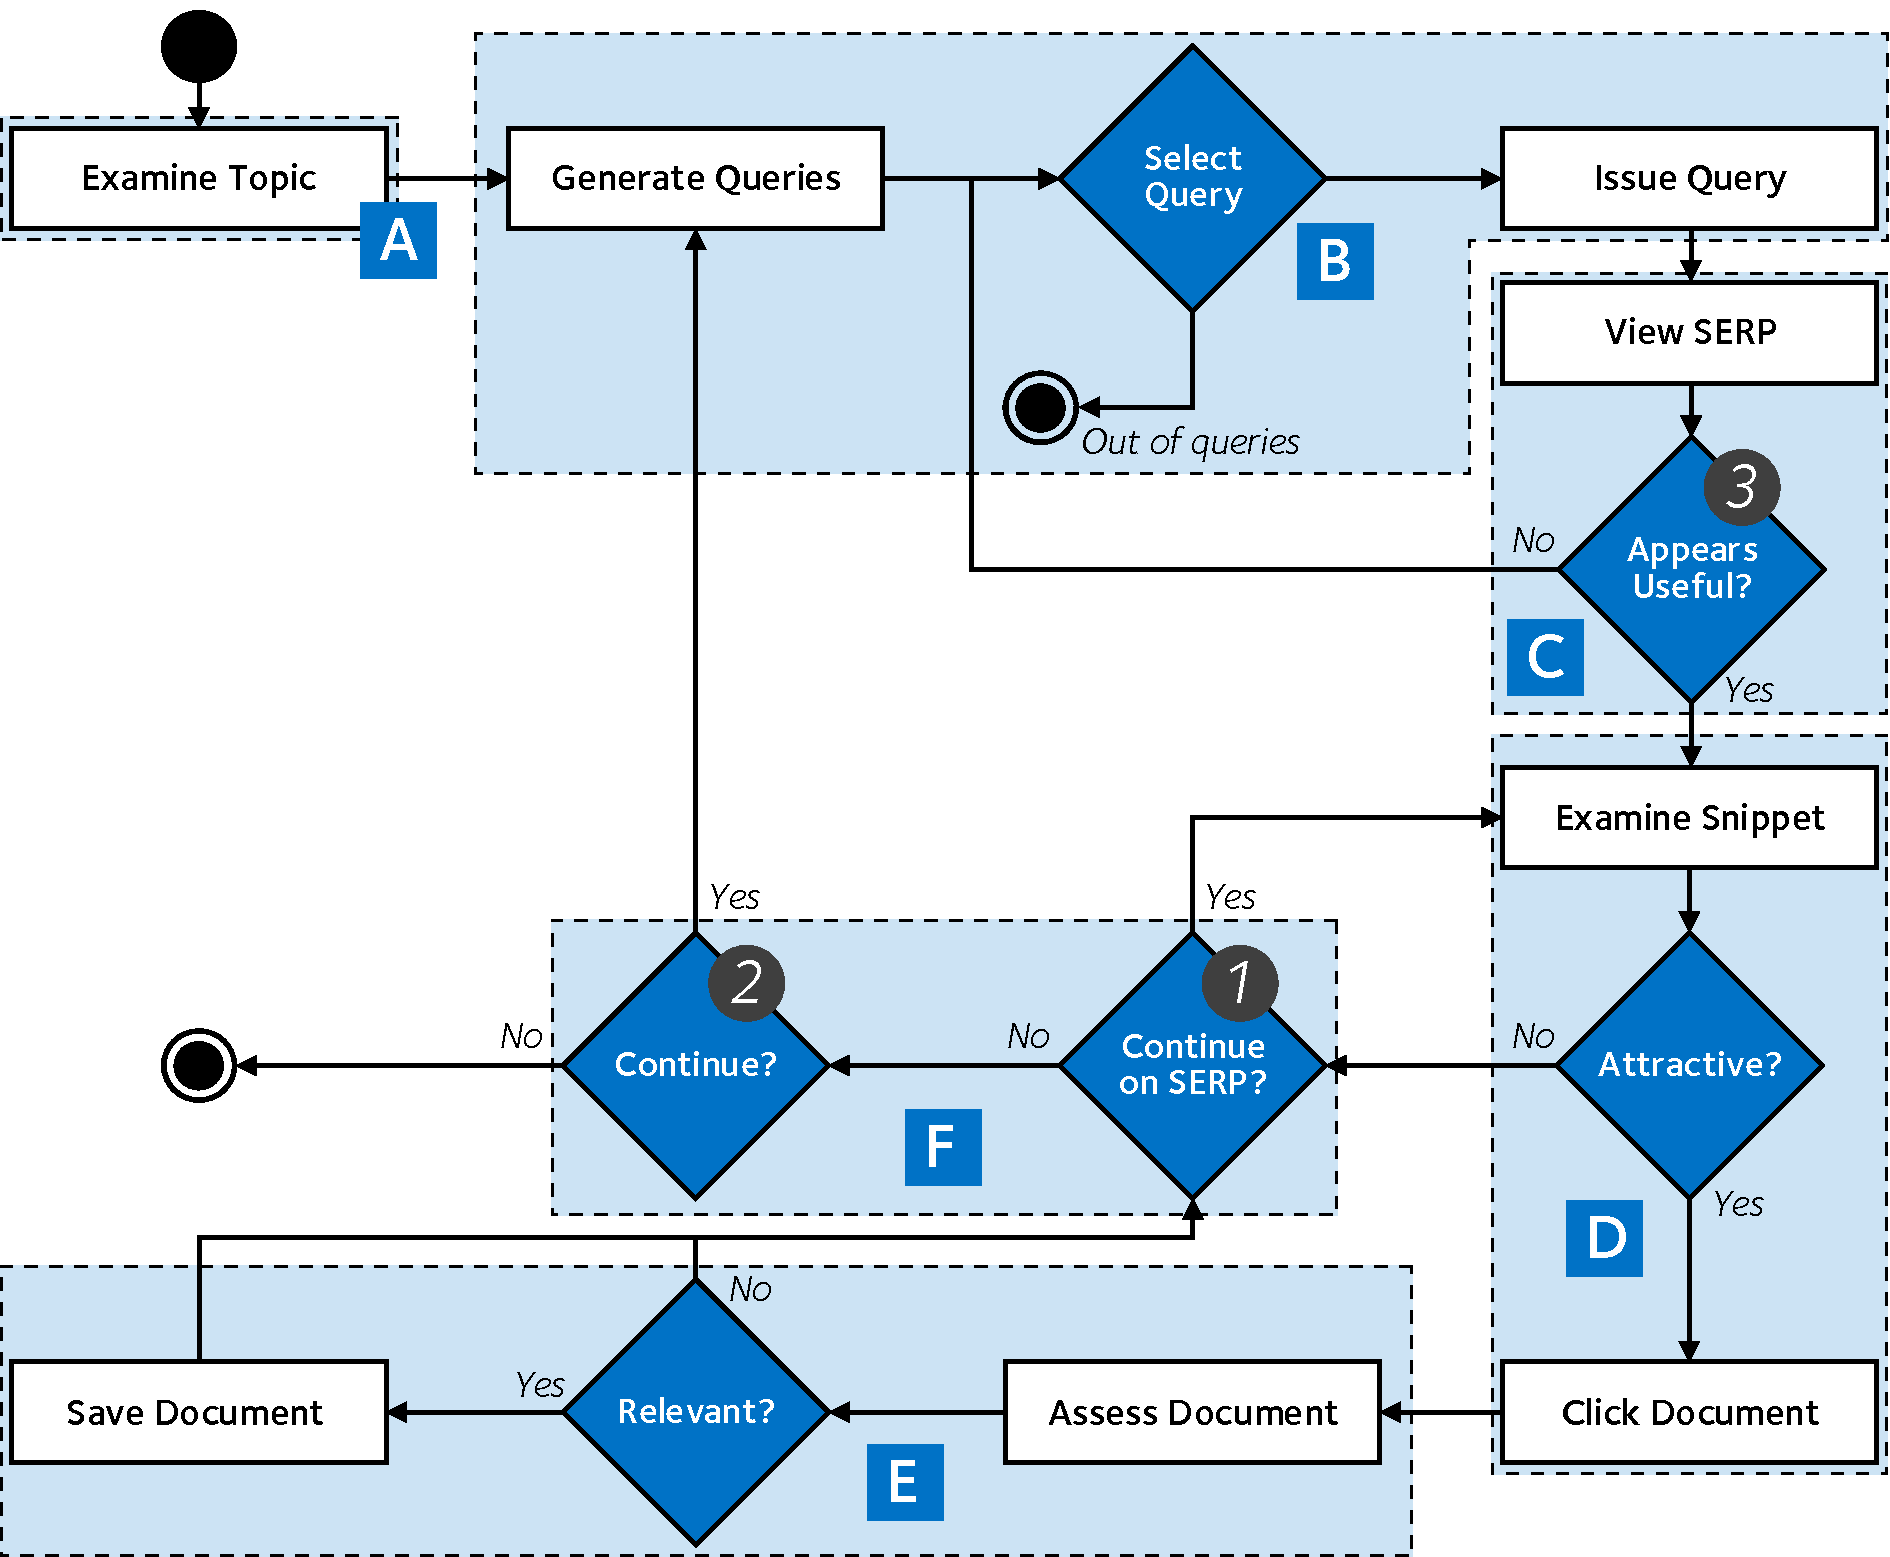
\includegraphics{figures/ch4-csm.pdf}}
    \caption[Flowchart of the~\glsfirst{acr:csm}]{A flowchart of the proposed~\glsfirst{acr:csm}, as used in experimental work discussed later in this thesis. Novel components that the work this thesis provides are highlighted by boxes \blueboxbold{A} and \blueboxbold{B}. The \emph{three} stopping decision points are highlighted with \blueboxbold{1}, \blueboxbold{2} and \blueboxbold{3} (refer to Section~\ref{sec:csm:stopping}). Refer to Section~\ref{sec:csm:csm:flow} for an in-depth explanation of the model.}
    \label{fig:csm}
\end{figure}

\subsection{Advancements}\label{sec:csm:csm:advancements}
The~\gls{acr:csm} provides two novel contributions to user modelling, both of which are discussed below.

\begin{itemize}
    \item{We provide advancements to the \blueboxbold{querying} aspects of the searcher model. In particular, a searcher subscribing to the~\gls{acr:csm} is able to generate an updated set of potential queries once he or she has completed interactions on a given~\gls{acr:serp}.}
    \item{\blueboxbold{\gls{acr:serp}} level stopping}
    
\end{itemize}

Mention the querying component. But don't go into too much detail about it.

\subsubsection{Querying Improvements}

\subsubsection{\gls{acr:serp} Level Stopping}


\subsection{Model Flow}\label{sec:csm:csm:flow}

\subsection{Stopping Decision Points}\label{sec:csm:csm:stopping}

\subsection{Model Assumptions}\label{sec:csm:csm:assumptions}

\section{Operationalised Stopping Strategies}\label{sec:csm:stopping}

\subsection{Fixed Depth}

\subsubsection{Considering Searcher Frustration and Satisfaction}

\subsubsection{Searcher Frustration}

\subsubsection{Goal/Satisfaction Based}

\subsubsection{Combining Frustration and Satisfaction}

\subsection{Considering the Difference}

\subsection{Considering Information Foraging Theory}

\subsubsection{Optimal Foraging}

\subsubsection{Time-Based Strategies}

\section{General Methodology Overview}\label{sec:csm:methodology}

\subsection{Conducing a User Study}

\subsection{Extracting User Study Interaction Data}

\subsection{Simulating Searcher Behaviours}

\subsection{Evaluating Performance and Searcher Approximations}

\section{Chapter Summary}